\subsection{CLAS12 Offline Software} \label{ssec:framework_clas12}

The CLAS12 Offline Software is the software associated to reconstructing the data detected at the CLAS12 detector from Hall B.
It is separated into two components: \textbf{common tools} and \textbf{reconstruction}~\cite{ziegler2013clas12}.

The \textbf{common tools} package is a set of libraries developed by the physicists at JLab that contain all the tools that are commonly reused by different engines, like the \textbf{detector geometry} or \textbf{magnetic fields} packages.
The \textbf{reconstruction} package, which is where most of this work is focused, is composed by a set of semi-independent engines connected via the aforementioned CLARA pipes, where each detector component is represented by one or more CLARA Data Processing Services.

These services are separated into two categories, ones that ``help'' the data flow (Event Builders, IO, etc) and others that describe the hardware of the CLAS12 detector.
A diagram of the detector can be seen in Figure \ref{fig:clas12_hardware_design}.

    \begin{figure}[h]
        \centering
        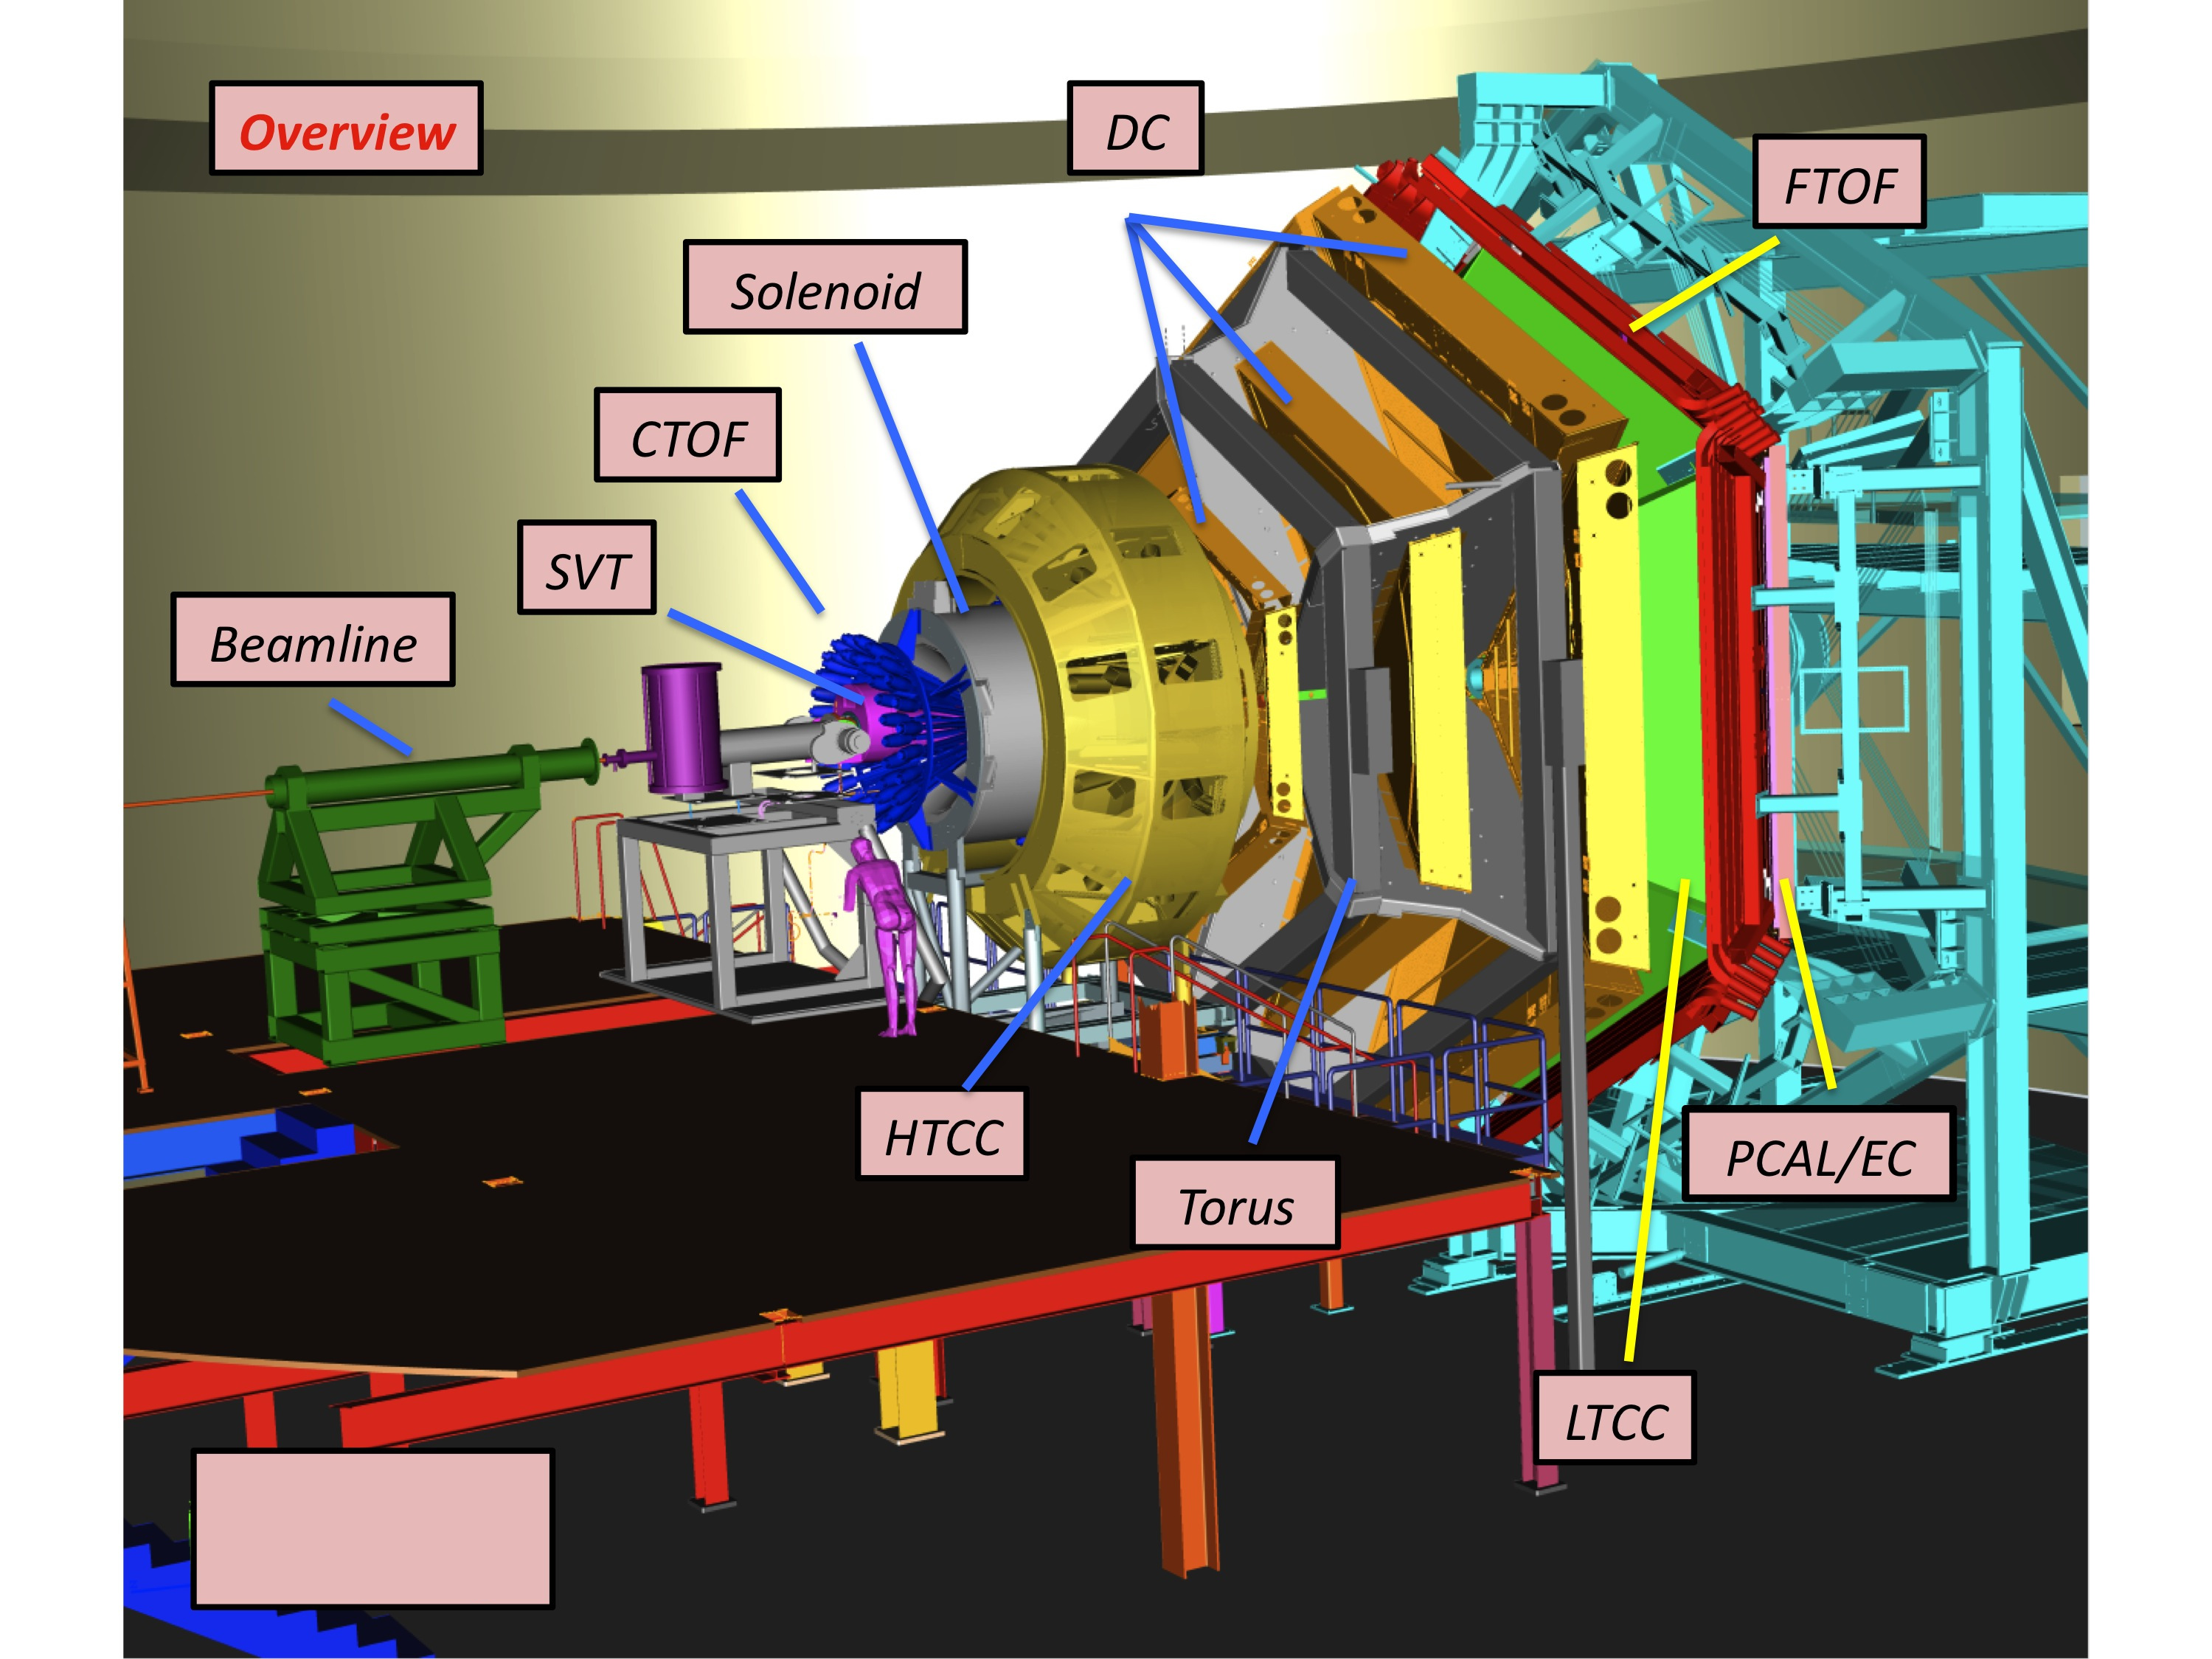
\includegraphics[scale=0.147]{clas12_hardware_design}
        \caption{\label{fig:clas12_hardware_design} CLAS12 detector hardware design. Source: CLAS12 web (\texttt{https://www.jlab.org/Hall-B/clas12-web/}).}
    \end{figure}

\newpage

A comprehensive list of CLAS12 software engines and their associated physical components (when available) is given.
It is worth noting that many engines run twice for each data event, first running a Hit-Based (HB) analysis and then a Time-Based (TB) analysis.
HB analysis is done without using time-related data and is mainly used to filter through the data and eliminate noise, while TB analyzes the filtered data and finds the final particle tracks.
    \begin{itemize}
        \item \textbf{HIPO READER and WRITER}: Engines that provide the file reading and writing, based on the HIgh Performance Output (HIPO) data format~\cite{gavalian2019data}. % Note: I could describe HIPO further, but it doesn't come in anytime during the whole thesis so idk.
        
        \item \textbf{Event Builder Hit-Based (EBHB) and Event Builder Time-Based (EBTB)}: Engines that build the data events from the HIPO data and pass them to the other engines.
        
        \item \textbf{MAGFIELDS}: Engine providing a model for the magnetic field inside the detector, used by components that need to estimate a particle's trajectory. % Note: I could describe how the magnetic field is simulated, but idk if it's really necessary.
        
        \item \textbf{High Threshold Cherenkov Counter (HTCC) and Low Threshold Cherenkov Counter (LTCC)}: Engines detecting particles moving faster than the local speed of light in a medium utilizing the emitted cone of light.
        The HTCC detects pions with high momenta ($>5~GeV/c$), while the LTCC the ones with low momenta ($>3~GeV/c$), and both are part of the Forward Detector (FD), a superconducting Torus magnet that covers the range from $5\degree$ to $40\degree$ measured from the source of the event, as can be seen in Figure \ref{fig:dc_horizontal_cut} from Section \ref{ssec:prob_context}.
        
        \item \textbf{DC Hit-Based tracking (DCHB) and Time-Based tracking (DCTB)}: The engines where most of the work in this thesis is focused, and are explained in detail in Section \ref{ssec:framework_dc}.
        Part of the FD.
        
        \item \textbf{Forward Time-Of-Flight Hit-Based detector (FTOFHB) and Time-Based detector (FTOFTB)}: Plastic scintillators that provide precise time-of-flight measurements for charged particle identification up to $4.5~GeV/c$.
        Scintillators are materials that show a scintillation or flash of light when excited by ionizing radiation.
        Part of the FD.
        
        \item \textbf{Ring Imaging Cherenkov (RICH) Detectors}: Similar in design to the FTOF detector, but capable of detecting charged particles with momenta of up to $8~GeV/c$ instead of $4.5$.
        Part of the FD.
        
        \item \textbf{Electromagnetic Calorimeter (EC)}: Allows for the detection of single high-energy photons by using a pre-shower calorimeter, improving spatial resolution and the separation of two photos for momenta of up to $10~GeV/c$.
        In particle physics, a shower refers to the cascade of secondary particles after the collision between the beam and the target.
        Part of the FD.
        
        \item \textbf{Central Time-Of Flight detector (CTOF)}: A scintillator array allowing for pion identification in a momentum range of up to $1.2~GeV/c$.
        Part of the Central Detector (CD), which is a superconducting Solenoid magnet that covers the polar angles from $35\degree$ to $135\degree$.
        
        \item \textbf{Central Neutron Detector (CND)}: A barrel with scintillator bars that detects high energy neutrons with an efficiency of up to $15\%$.
        The efficiency of a neutron detector refers to how many neutrons that pass through it are detected~\cite{pinchoff2005introduction}.
        Part of the DC.
        
        \item \textbf{Forward Tagger (FT) electromagnetic calorimeter (FTCAL), FT tracker (FTEB) and FT scintillation counter (FTHODO)}: An extension of the CLAS12 capabilities that allows it to detect electrons and photons at angles as low as $2.5\degree$.
        
        \item \textbf{Silicon Vertex Tracker (SVT) and Barrel Micromegas Tracker (BMT)}: Reconstruct the trajectories of charged tracks in the angular region from $35\degree$ to $125\degree$ with a momenta up to $1~GeV/c$.
        In the code, both components are contained inside the CVT engine.
    \end{itemize}

The production chain integrating all of the engines that represent these detectors can be seen in Figure \ref{fig:engines-chain}.

    \begin{figure}[h]
        \centering
        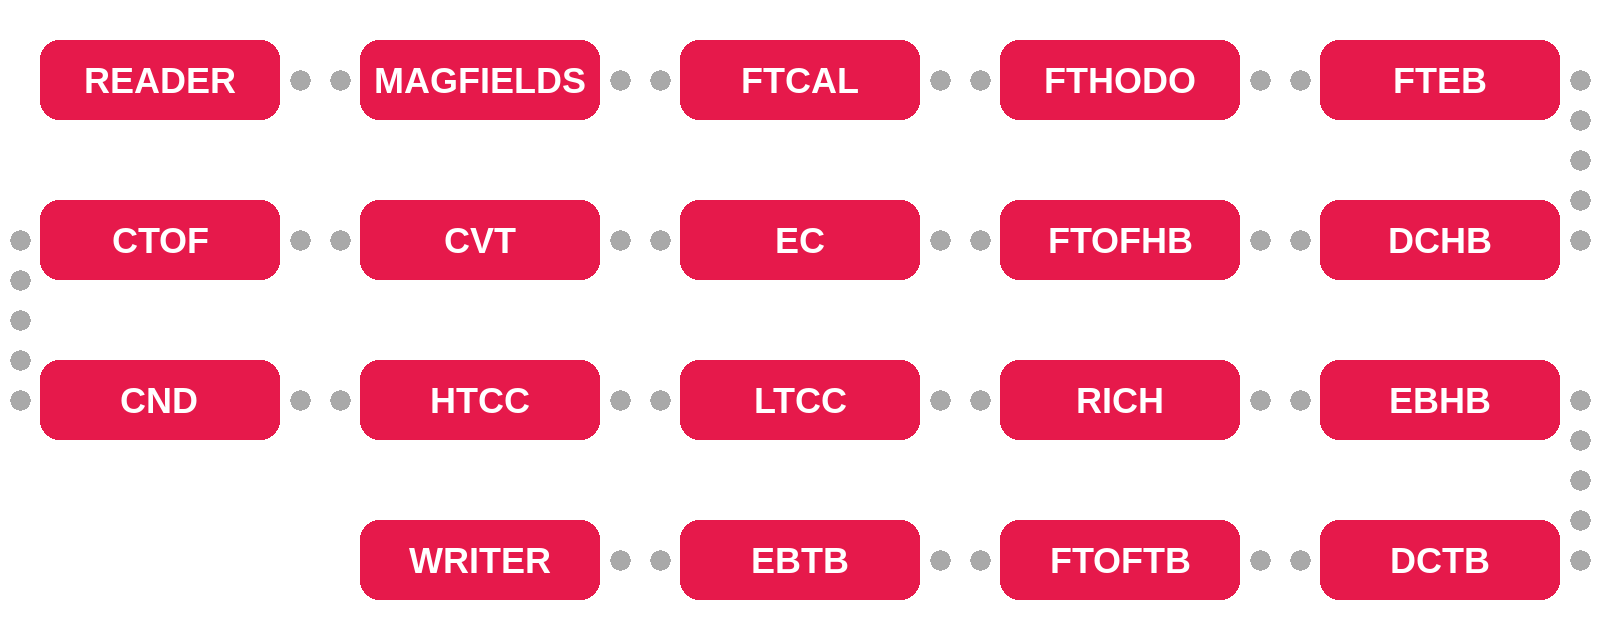
\includegraphics[scale=0.27]{engines_chain.png}
        \caption{\label{fig:engines-chain} CLAS12 engines production chain.}
    \end{figure}
    
\newpage